\documentclass[twoside]{AiTeX}
\usepackage{enumerate}

\lstdefinestyle{customVHDL}{
  backgroundcolor=\color{backcolour},   
    commentstyle=\color{codegreen},
    keywordstyle=\color{magenta},
    numberstyle=\tiny\color{codegray},
    stringstyle=\color{codepurple},
    basicstyle=\ttfamily\footnotesize,
    breakatwhitespace=false,         
    breaklines=true,                 
    captionpos=b,                    
    keepspaces=true,                 
    numbers=left,                    
    numbersep=5pt,                  
    showspaces=false,                
    showstringspaces=false,
    showtabs=false,                  
    tabsize=2,
    xleftmargin=\parindent,
    language=vhdl,
    emph={%  
     = ,  <= %
    },emphstyle={\color{magenta}}%
}


\begin{document}
%\datos{facultad}{universidad}{grado}{asignatura}{subtitulo}{autor}{curso}
\datos{Informática}{Universidad Complutense de Madrid}{Ingeniería informática}{Tecnología y Organización de Computadores}{Cómo diseñar circuitos para el mercado y aprender la importancia del diseño en el rendimiento final del dispositivo }{Alejandro Barrachina Argudo}{2020-2021}
\portadaApuntes
%\pagestyle{empty}
\tableofcontents
\justify
\pagestyle{fancy}
\chapterA{Modelado hardware con VHDL. Introducción a las FPGAs}
\section{Flujo de diseño}

TODO

\section{Lenguaje de descripción hardware}
\gls{hdl} es un lenguaje específicamente creado para el diseño de circuitos, tanto a nivel de puerta como a nivel e comportamiento. La estructura del lenguaje sugiere el diseño \gls{hw}.

Los \gls{hdl} se usan para poder descubrir problemas en el diseño del \gls{hw} antes de su implementación física. Como la complejidad de los sistemas electrónicos crece exponencialmente, es necesaria una herramienta que trabaje con el ordenador. Por último, gracias a estas herramientas más de una persona puede trabajar en el mismo proyecto

En este curso usaremos \gls{vhdl}, esto nos permite hacer descripciones de la estructura del circuito con:
\begin{itemize}
	\item Descomposición en sub-circuitos
	\item Interconexión de sub-circuitos
	\item comportamiento
	\item Estructural
\end{itemize}
También permite la especificación de un circuito utilizando formas familiares de lenguajes de programación y la simulación del circuito antes de su fabricación.

Un \gls{hdl} tiene que ser capaz de simular el comportamiento real del \gls{hw} sin que el programador necesite imponer restricciones.

\noindent \textbf{Ejemplo 1:}

\begin{table}[H]
	\centering
	\begin{tabular}{|l|l|}
		\hline
		\cellcolor[HTML]{70A9FC} t = 5ns & \cellcolor[HTML]{70A9FC} t=10ns \\ \hline
		A = 0                            & A = 1                           \\ \hline
		B = 1                            & B = 1                           \\ \hline
		C = 0                            & C = 0                           \\ \hline
	\end{tabular}
\end{table}

\begin{multicols}{2}
	\underline{Descripción 1:}

	D = A and B;

	S = D or C;

	\columnbreak

	\underline{Descripción 2:}

	S = D or C;

	D = A and B;
\end{multicols}

\textcolor{cyan}{?`Se obtiene el mismo resultado?} No, en la descripción 1 en t = 10ns el valor de S será 1, mientras que en la descripción 2 seguirá siendo 0.


\newpage
\section{Simulación con VHDL}
\gls{vhdl} realiza la simulación siguiendo la técnica de \textbf{simulación por eventos discretos}, esto permite avanzar el tiempo a intervalos variables, en función de la planificación de ocurrencia de eventos.
La simulación consta de tres fases:
\begin{itemize}
	\item\textbf{Fase 0: }fase de inicialización donde las señales se les asignan unos valores iniciales y se pone el tiempo a cero. La asignación se hace rellenando una lista de eventos para el instante t = 0.
	\item\textbf{Fase 1: }todas las transiciones planificadas para ese tiempo se ejecutan
	\item\textbf{Fase 2: }las señales que se han modificado en consecuencia de las transiciones planificadas en el instante t se escriben en la lista de eventos planificándose para el instante t + $\delta$, donde $\delta$ es un instante infinitesimal. Una vez acabado esta fase se vuelve a la fase 1 hasta que se termine la simulación.
\end{itemize}

\begin{multicols}{3}
	\begin{figure}[H]
		\centering
		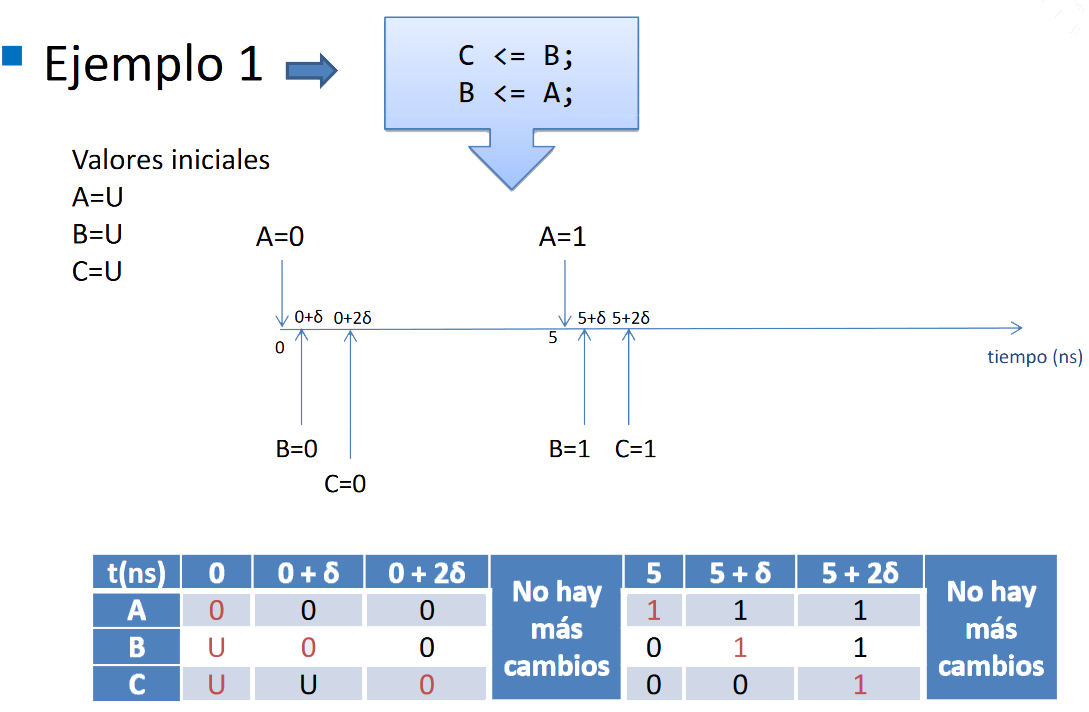
\includegraphics[width=0.3\textwidth]{images/Tema_1/VHDL_Ejemplo_1.PNG}
	\end{figure}
	\vfill
	\begin{figure}[H]
		\centering
		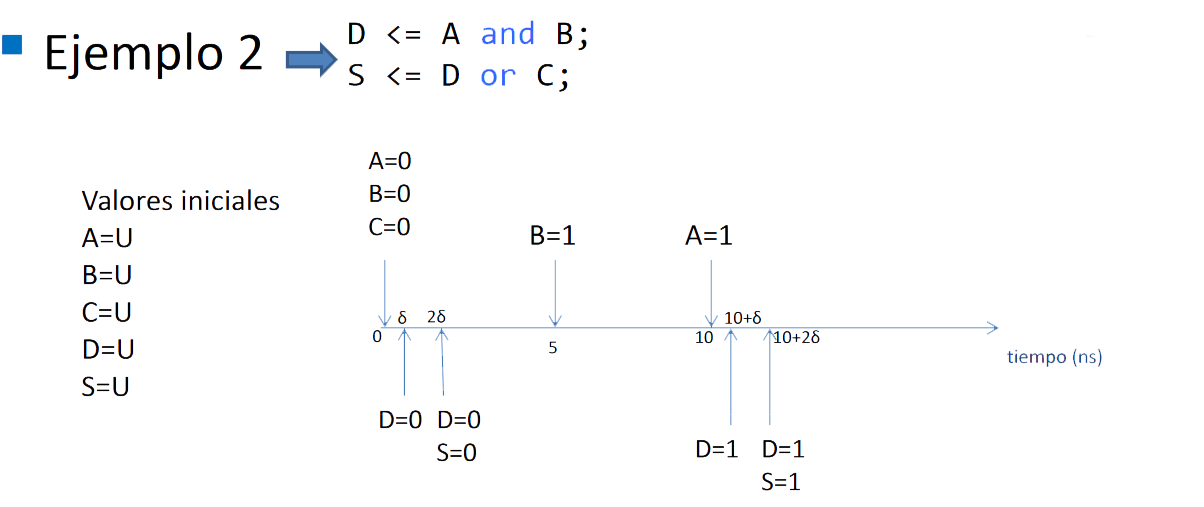
\includegraphics[width=0.3\textwidth]{images/Tema_1/VHDL_Ejemplo_2.PNG}
	\end{figure}
	\vfill
	\begin{figure}[H]
		\centering
		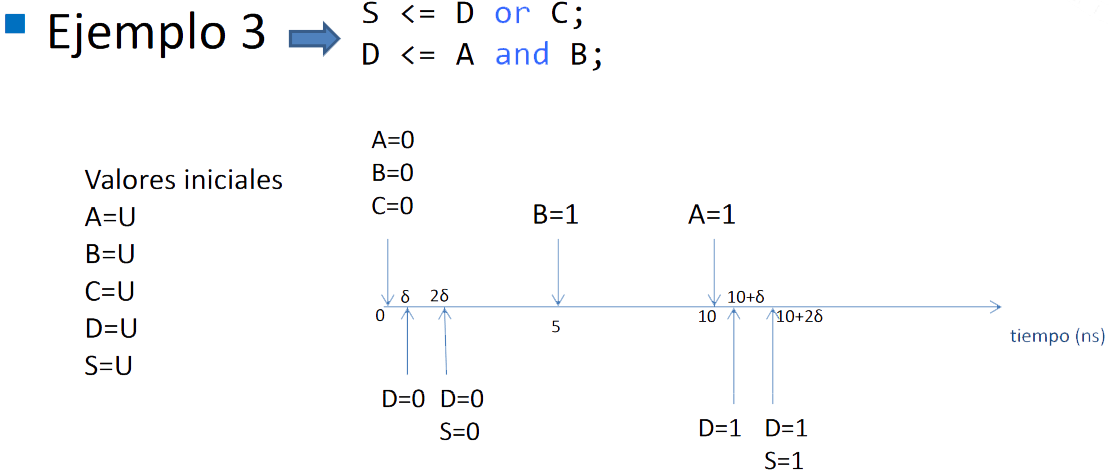
\includegraphics[width=0.3\textwidth]{images/Tema_1/VHDL_Ejemplo_3.PNG}
	\end{figure}
\end{multicols}


\textbf{Pregunta ejemplo 3: }?`Qué pasaría si en 5 en vez de cambiar B cambia C? S=1 ya que D or C si c = 1 siempre es 1.


\section{Estructura de un modelo VHDL}
Un sistema digital está descrito por sus entradas y sus salidas, donde las salidas dependen de las entradas.
Los modelos \gls{vhdl} están formados por dos partes:
\begin{multicols}{2}
	\begin{figure}[H]
		\centering
		\lstinputlisting[style=customVHDL]{Code/Tema_1/Ejemplo_Entity_1.vhd}
		\caption{Ejemplo Entity}
	\end{figure}
	\vfill
	\begin{figure}[H]
		\centering
		\lstinputlisting[style=customVHDL]{Code/Tema_1/Ejemplo_Architecture_1.vhd}
		\caption{Ejemplo Architecture}
	\end{figure}
\end{multicols}

La entity define externamente el circuito o subcircuito,  especifica el nombre y el número de puertos, su tipo de datos y si son de entrada o salida, tiene toda la información necesaria para conectar tu circuito a otros circuitos.
La architecture define internamente el circuito, sus señales internas, funciones, procedimientos, constantes, etc.


Cada architecture va asociada a una entity y se indica en la primera sentencia. Antes del begin se definen las señales, los tipos y los componentes

\begin{figure}[H]
	\centering
	\lstinputlisting[style=customVHDL]{Code/Tema_1/Ejemplo_completo_1.vhd}
	\caption{Ejemplo Entity y Architecture}
\end{figure}

\section{Elementos básicos de VHDL}

Las sentencias concurrentes siempre se encuentran fuera de los PROCESS, aparecen en cualquier punto del programa después del begin de la arquitectura,  es lógica combinacional pura y siempre tiene un ELSE final o un WHEN OTHERS.

\begin{multicols}{2}
	\begin{figure}[H]
		\centering
		\lstinputlisting[style=customVHDL]{Code/Tema_1/Ejemplo_When-Else.vhd}
		\caption{Ejemplo When-Else}
	\end{figure}
	\vfill
	\begin{figure}[H]
		\centering
		\lstinputlisting[style=customVHDL]{Code/Tema_1/Ejemplo_When-Select-Else.vhd}
		\caption{Ejemplo With-Select-Else}
	\end{figure}
\end{multicols}


Los procesos son sentencias concurrentes. Solo se ejecutan esas sentencias que se encuentran dentro del proceso si alguna de las señales de la lista de sensibilidad ha cambiado de valor. La lista de sensibilidad es opcional, si no existe el proceso se ejecuta infinitas veces. Es un código secuencial.
\begin{figure}[H]
	\centering
	\lstinputlisting[style=customVHDL, xleftmargin=.2\textwidth, xrightmargin=.2\textwidth]{Code/Tema_1/Ejemplo_Process.vhd}
	\caption{Ejemplo Process}
\end{figure}

Las secuencias condicionales van dentro de un process, si la lista de sensibilidad está incompleta, el comportamiento del process será incorrecto. Estas sentencias deben tener un caso por defecto.
\begin{multicols}{2}
	\begin{figure}[H]
		\centering
		\lstinputlisting[style=customVHDL]{Code/Tema_1/Ejemplo_If-Then-Else.vhd}
		\caption{Ejemplo If-Then-Else}
	\end{figure}
	\vfill
	\begin{figure}[H]
		\centering
		\lstinputlisting[style=customVHDL]{Code/Tema_1/Ejemplo_Case.vhd}
		\caption{Ejemplo Case}
	\end{figure}
\end{multicols}

Ejemplos de bucles en VHDL:
\begin{multicols}{3}
	\begin{figure}[H]
		\centering
		\lstinputlisting[style=customVHDL]{Code/Tema_1/Ejemplo_Loop_1.vhd}
		\caption{Loop simple}
	\end{figure}
	\vfill
	\begin{figure}[H]
		\centering
		\lstinputlisting[style=customVHDL]{Code/Tema_1/Ejemplo_For_Loop.vhd}
		\caption{For Loop}
	\end{figure}
	\vfill
	\begin{figure}[H]
		\centering
		\lstinputlisting[style=customVHDL]{Code/Tema_1/Ejemplo_While_Loop.vhd}
		\caption{While Loop}
	\end{figure}
\end{multicols}

Las sentencias wait se usan en procesos, procedimientos y funciones y, como indica su nombre, hace que haya un tiempo de espera. Puede ser de tres tipos:
\begin{itemize}
	\item\textbf{wait for} <timeout clause, time delay>: \textcolor{magenta}{wait for} 10 ns;
	\item\textbf{wait until} <condition>: \textcolor{magenta}{wait until} clk = '1';
	\item\textbf{wait on} <sensitive clause, event>: \textcolor{magenta}{wait on} in1;
\end{itemize}


Atributos:
\begin{itemize}
	\item S'\textbf{DELAYED}(t) es el valor de la señal S en el tiempo actual -t.
	\item S'\textbf{STABLE} es true si no hay ningún evento ocurriendo para S.
	\item S'\textbf{STABLE}(t) es true si no hay eventos ocurriendo en S durante t unidades de tiempo.
	\item S'\textbf{QUIET} es true si no hay eventos en ese ciclo de simulación para la señal S.
	\item S'\textbf{QUIET}(t) es true si no hay eventos en ese ciclo de simulación para la señal S durante t unidades de tiempo.
	\item S'\textbf{TRANSACTION} es un valor BIT, el inverso del valor previo de cada ciclo en que S está activo.
	\item S'\textbf{EVENT} es true si S tiene un evento en el ciclo de simulación.
	\item S'\textbf{ACTIVE} es true si S está activa durante el ciclo de simulación.
	\item S'\textbf{LAST\_EVENT} es el tiempo desde el último evento en S.
	\item S'\textbf{LAST\_ACTIVE} es el tiempo desde la última vez que S estuvo activa.
	\item S'\textbf{LAST\_VALUE} es el valor anterior de S.
\end{itemize}

Tipos de datos:
\begin{itemize}
	\item Tipos enteros y reales:
	      \begin{itemize}
		      \item INTEGER
		      \item NATURAL
		      \item REAL
	      \end{itemize}
	\item Tipos físicos
	      \begin{itemize}
		      \item TIME
		      \item RESISTANCE
	      \end{itemize}
	\item Tipos enumerados: conjuntos de posibles valores
	      \begin{itemize}
		      \item BIT {0,1}
		      \item BOOLEAN {TRUE, FALSE}
		      \item CHARACTER {ASCII CHARACTERS}
		      \item STD\_LOGIC {U, X, 0, 1, Z, W, L, H, -}
	      \end{itemize}
\end{itemize}

Se pueden definir tipos personalizados

\begin{figure}[H]
	\centering
	\lstinputlisting[style=customVHDL]{Code/Tema_1/Ejemplo_Tipos_Personalizados.vhd}
	\caption{Ejemplo tipos personalizados}
\end{figure}

Arrays:

\begin{figure}[H]
	\centering
	\lstinputlisting[style=customVHDL]{Code/Tema_1/Ejemplo_Arrays.vhd}
	\caption{Ejemplo Arrays}
\end{figure}

Un \textbf{componente} es una entidad que se describe dentro de una arquitectura
\begin{figure}[H]
	\centering
	\lstinputlisting[style=customVHDL, xleftmargin=.2\textwidth, xrightmargin=.2\textwidth]{Code/Tema_1/Ejemplo_Component.vhd}
	\caption{Ejemplo Component}
\end{figure}


\textbf{Generate:} las secuencias de generación de componentes permiten crear una o más copias de un conjunto de interconexiones, lo cual facilita el diseño de circuitos mediante descripciones estructurales

\begin{figure}[H]
	\centering
	\lstinputlisting[style=customVHDL, xleftmargin=.2\textwidth, xrightmargin=.2\textwidth]{Code/Tema_1/Ejemplo_Generate.vhd}
	\caption{Ejemplo Generate}
\end{figure}

Un \textbf{paquete} son agrupaciones de tipos, funciones y procedimientos personalizados. Pueden ser incluidos en uno o varios diseños, normalmente se definen en ficheros .vhd dedicados.

\begin{figure}[H]
	\centering
	\lstinputlisting[style=customVHDL, xleftmargin=.2\textwidth, xrightmargin=.2\textwidth]{Code/Tema_1/Ejemplo_Package.vhd}
	\caption{Ejemplo Package}
\end{figure}

\section{Entidades parametrizables}
Una entity puede tener una lista de parámetros. El valor por defecto de los parámetros genéricos es opcional, sin embargo, no se puede sintetizar un diseño con parámetros que no tengan asignado un valor.

Al instanciar este componente en otro fichero, hay que asignar un valor a n si y solo si no se le dio un valor por defecto en su declaración de entity.

Se  puede  utilizar  la  asignación (others=> ‘0’) o (others=> ‘1’) para asignar el valor “0...0” o “1...1” a una señal de longitud parametrizable.

\section{Testbench de simulación}
Para conocer si nuestro diseño funciona correctamente tendremos que introducir unos estímulos en las entradas y comprobar que las salidas obtenidas son las deseadas.

\textbf{Estructura básica:}
\begin{enumerate}
	\item Se crea una entidad de simulación sin puertos de entrada ni de salida
	\item Se añade como component la entity a verificar
	\item Se definen tantas señales como puertos de la entity del diseño a verificar
	\item Se instancia el component igualando las señales internas a las entradas
	\item Se crea el process de simulación, no tiene lista de sensibilidad
	\item Se definen los valores iniciales de las entradas
	\item Se definen los valores de las entradas en los siguientes instantes de tiempo
\end{enumerate}

Cómo implementar una entrada periódica: clk
\begin{figure}[H]
	\centering
	\lstinputlisting[style=customVHDL, xleftmargin=.2\textwidth, xrightmargin=.2\textwidth]{Code/Tema_1/Ejemplo_Clk.vhd}
	\caption{Ejemplo Clk}
\end{figure}

Como este process no acaba con un wait sin for, se repetirá indefinidamente.


\section{Introducción a las FPGAs}
Una \gls{fpga} es un \gls{hw} de prototipado automático. Inicialmente servía para lo mismo que un entrenador, con la diferencia de que el circuito se implementaba automáticamente. Debido a su gran capacidad de procesamiento, versatilidad y a las herramientas de diseño 9. Introducción a las TC versatilidad y a las herramientas de diseño disponibles, actualmente existen circuitos comerciales que llevan \gls{fpga} incorporadas.

Los componentes de una \gls{fpga} son:
\begin{itemize}
	\item Celdas de entrada salida
	\item Celdas lógicas programables
	\item Celdas de interconexión programables (las estructuras de interconexionado son muy costosas)
	\item Memorias(opcional)
	\item Multiplicadores(opcional)
	\item Micro-controladores(opcional)
\end{itemize}

Una CLB contiene:
\begin{itemize}
	\item Look-Up Tables: son memorias \gls{rom} que almacenan 1x16 bits, pueden implementar cualquier función lógica de 4 entradas.
	\item Biestables: se utilizan en el caso de que la celda deba implementar \gls{hw} secuencial. Se pueden configurar si son disparados por flanco o por nivel.
	\item Multiplexores: para interconectar las entradas con los módulos o los módulos entre si se utilizan multiplexores
\end{itemize}
%finished
\chapterA{Evaluación de parámetros físicos del diseño}
\section{Parámetros}
\textbf{Área (tamaño).} Tamaño de silicio ($cm^{2}$ o $mm^{2}$) necesarios para implementar una determinada aplicación. Depende de la arquitectura del circuito y de la tecnología empleada para su fabricación. Si no tenemos el layout del circuito podemos estimarlo con un número de puertas NAND equivalente.\\
\textbf{Velocidad (tiempo).} La velocidad de un circuito se corresponde con el tiempo necesario para realizar una determinada función, normalmente este concepto se calcula sobre el peor caso posible. Siempre es deseable que el circuito sea lo más rápido posible, pero casi siempre para conseguirlo se necesita un diseño más sofisticado, lo que puede implicar un mayor área de silicio y/o un mayor consumo de energía. La velocidad de un circuito está directamente relacionada con la frecuencia de reloj, pero no es verdad que una mayor frecuencia de reloj garantice que el resultado se obtenga en menos tiempo. Tendremos que evaluar a qué frecuencia puede trabajar el circuito, cuántas operaciones puede realizar por unidad de tiempo y si funcionará correctamente a la frecuencia de reloj exigida.\\
\textbf{Potencia (energía).} La potencia hace referencia a la energía consumida por el circuito al realizar las operaciones para las cuales fue diseñado. En todos aquellos circuitos diseñados para dispositivos móviles la reducción del consumo de potencia es la prioridad. Antes de su fabricación el circuito puede ser rediseñado para cumplir los requisitos de consumo. Un mismo diseño consume menos en tecnologías. La temperatura que alcanza un circuito está directamente relacionada con el consumo de energía. Cuanto mas dure la batería de un circuito, menor será el impacto medioambiental. \\
\textbf{Coste.} El diseño de un circuito digital es rara vez un objetivo en sí mismo. Se trata de una actividad económica y el coste es un importante factor, si no el decisivo.
En el coste final del circuito influyen:
\begin{itemize}
	\item El coste de desarrollo (diseño)
	\item El coste de producción (diseño y fabricación)
	\item El tiempo de salida al mercado (comercialización)
\end{itemize}


La importancia de la evaluación es:
\begin{itemize}
	\item Conseguir diseños más rápidos, con mayor capacidad de procesamiento y reducción en la cantidad de recursos hardware para realizar las mismas operaciones.
	\item Diseños más pequeños, menor coste de fabricación, menor posibilidad de errores físicos durante la fabricación y aumentar la capacidad de integración.
	\item Diseños más eficientes energéticamente, con menor huella de $CO_{2}$, mayor duración de la batería y menor coste de operación.
\end{itemize}

\section{Análisis estático de tiempos (STA)}
El análisis de la temporización de un circuito recibe el nombre de \gls{sta}. Determina si el circuito satisface los requisitos de temporización impuestos por el reloj.
\\ Para este análisis debemos calcular el retardo de todos los caminos del circuito y determinar si su valor es mayor o menor que el valor límite impuesto por la señal de reloj. Si es mayor el retardo, entonces se produce una violación del timing. Si es menor, entonces el camino más lento establece la frecuencia máxima del reloj.

\subsection{Retardo de camino}
Es la suma de los retardos de la lógica y conexiones desde:
\begin{itemize}
	\item Las entradas primarias hasta las salidas primarias para todos los posibles caminos combinacionales.
	\item Las entradas primarias hasta los elementos de memoria.
	\item Los elementos de memoria hasta las salidas primarias.
	\item Desde los elementos de memoria hasta los elementos de memoria.
\end{itemize}
\textcolor{blue}{Retardo de lógica}: retardo de las puertas o elementos lógicos del circuito.
\begin{itemize}
	\item Combinacionales. OR, AND, sumadores, decodificadores\dots
	\item Secuenciales: FF, contadores, registros, memorias \dots
\end{itemize}
\textcolor{blue}{Retardo de conexión}: todas las conexiones del circuito tienen un retardo.

\subsection{Modelado retardo: timing arcs}
Combinacional: retardo desde cualquier entrada a cualquiera de sus salidas. Secuencial: retardo desde el pin del reloj hasta cualquiera de sus salidas, a este tiempo se le conoce como Clk-2-Q. Conexiones: retardo desde el pin de salida hasta cada uno de sus destinos.
\section{Cálculo de tiempo de propagación}
Se suman todos los retardos de la lógica y las conexiones para todos los caminos del circuito  combinacional. Depende del camino, hay tantos tiempos como caminos. Se usa el valor del camino más lento, conocido como \textbf{camino crítico.}
\subsection{Funcionamiento síncrono}
Si en el sistema hay elementos de memoria debe existir un reloj. El reloj determina cuándo se actualiza el estado de los elementos de memoria del sistema.\\
La hipótesis de funcionamiento síncrono obliga a que la diferencia en tiempo entre dos flancos consecutivos (positivos o negativos los dos) sea superior al tiempo necesario para que los valores de las entradas de los registros sean estables.
\subsection{Definiciones}
\noindent\textbf{Tiempo de set-up:} tiempo mínimo que la entrada debe permanecer antes del suceso del reloj.\\
\textbf{Tiempo de hold:} tiempo mínimo que la entrada debe permanecer estable después del suceso del reloj.\\
\textbf{Tiempo de propagación del registro:} tiempo que tarda en propagarse el dato desde la entrada hasta la salida del registro cuando ocurre el flanco activo de reloj.\\
\textbf{Tiempo de propagación combinacional:} tiempo desde que cambian las entradas del circuito combinacional hasta que se produce un cambio en las salidas. Depende del camino. Se usa el valor del camino crítico.\\
\begin{multicols}{2}
	\begin{figure}[H]
		\centering
		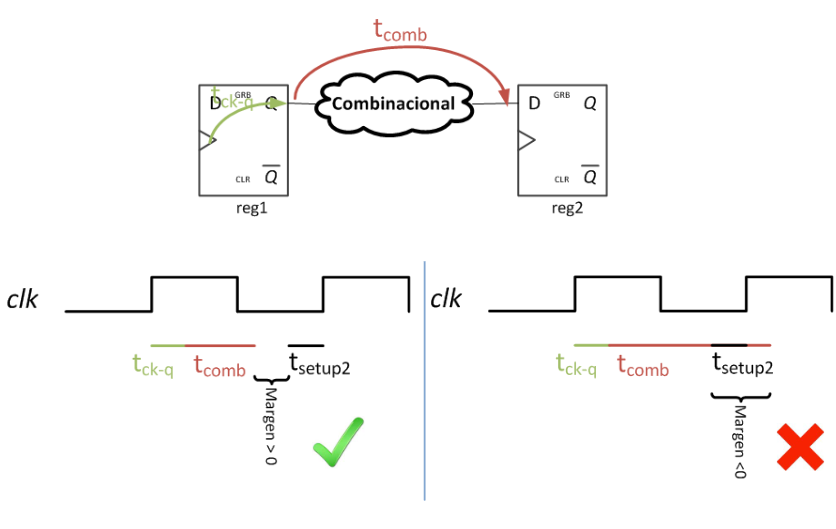
\includegraphics[width=0.4\textwidth]{images/Tema_2/Margen_setup.PNG}
		\caption{Margen de setup}
	\end{figure}
	\vfill
	\null
	\begin{figure}[H]
		\centering
		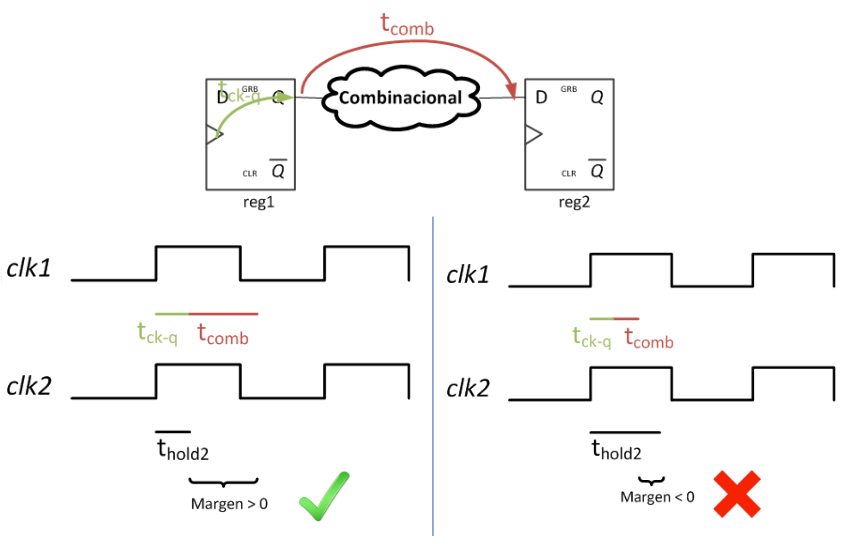
\includegraphics[width=0.4\textwidth]{images/Tema_2/Margen_hold.PNG}
		\caption{Margen de setup}
	\end{figure}
\end{multicols}
\subsection{Cálculo de tiempo de set-up y hold}
Sin considerar el clock skew y el clock jitter:
\[
	Margen\; setup = t_{clk}- \left(t_{clk_q} +t_{comb} + t_{setup}\right)
\]
\[
	Margen \; hold = t_{clk_q} + t_{comb} + t_{hold}
\]
Margen negativo $\rightarrow$ \textcolor{red}{error de temporización}
\begin{figure}[H]
	\centering
	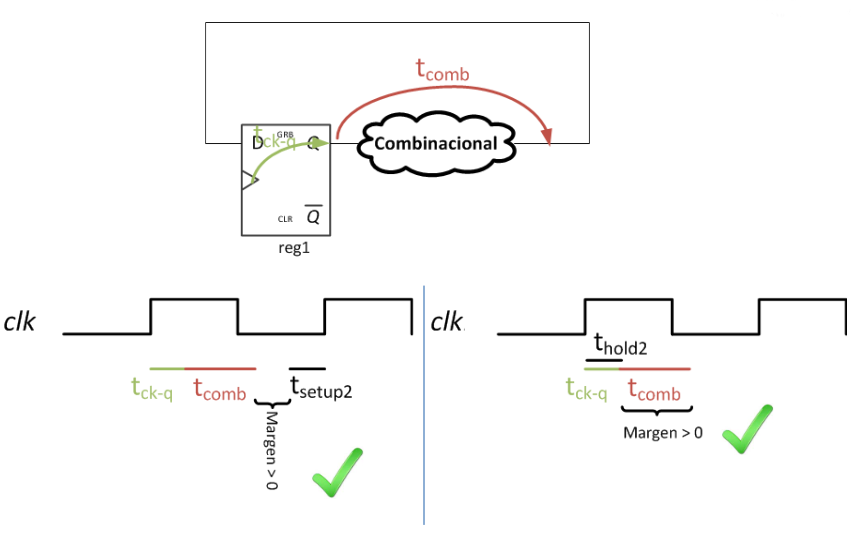
\includegraphics[width=0.8\textwidth]{images/Tema_2/Circ_retroalimentado.PNG}
	\caption{Circuito retroalimentado}
\end{figure}

\subsection{Metaestabilidad}
Consiste en una indecisión prolongada en el comportamiento lógico del  biestable al intentar almacenar uno de sus dos estados estables.
Ocurre si existe una violación de setup o de hold. Mientras ese biestable permanezca en metaestabilidad, sus señales de salida están indefinidas a nivel lógico.
\subsection{Clock skew}
El sesgo del reloj es un fenómeno que ocurre en los circuitos secuenciales cuando el reloj no llega al mismo tiempo a todos los componentes de memoria. Puede deberse a la longitud del cable, variaciones de temperatura, capacidades parásitas, imperfecciones del silicio, etc.
Cuando el tiempo de ciclo es pequeño, este problema se convierte en uno de los más importantes a la hora de diseñar el circuito.\\
Hay dos tipos de clock skew:
\begin{itemize}
	\item\textbf{Positive skew:} el registro que transmite recibe el reloj antes que el registro que recibe.
	\item\textbf{Negative skew:} el registro que transmite recibe el reloj después que el registro que recibe.
\end{itemize}
\[
	skew=t_{dest}-t_{orig}
\]

\subsection{Clock jitter}
El jitter es una modificación no deseada en la periodicidad del reloj. En otras palabras, es la variación de los flancos de reloj respecto de su posición ideal en el tiempo.
Tiene orígenes muy variados, variaciones en la fabricación de los osciladores, variaciones de temperatura etc.\\
Se especifica de tres maneras:
\begin{itemize}
	\item\textbf{Jitter absoluto:} diferencia entre la posición real del flanco de reloj y su posición ideal.
	\item\textbf{Jitter periódico:} diferencia entre el periodo real del reloj y el periodo ideal. Es el más importante a efectos de STA
	\item\textbf{Jitter ciclo-a-ciclo:} diferencia en la duración de dos periodos de reloj adyacentes
\end{itemize}

Es necesario tenerlo en cuenta en el análisis temporal del circuito porque puede acortar la duración del ciclo de reloj. Especificado como RMS(Root Mean Square) o valor pico-a-pico, se mide la duración media del ciclo sobre una muestra y se obtiene su desviación estándar.

\subsection{Cálculo de tiempo de setup y hold}
Considerando el clock skew y el clock jitter
\[
	Margen\; setup = t_{clk} + skew - \left(t_{clk\_q} + t_{comb} + t_{setup} + jitter\right)
\]
\[
	Margen\; hold = t_{clk\_q} + t_{comb} - \left(skew + jitter + t_{hold}\right)
\]
Margen negativo $\rightarrow$ \textcolor{red}{error de temporización}
\[
	t_{clk} + skew > \left(t_{clk\_q} + t_{comb} + t_{setup} + jitter\right)
\]
\[
	t_{clk} > \left(t_{clk\_q} + t_{comb} + t_{setup} + jitter\right) -skew
\]

\subsection{Falso camino crítico}
Parece el camino más lento del circuito pero en realidad no lo es, no propaga una transición. Los diseños que comparten lógica para distintos cálculos son susceptibles de tener falsos caminos.

\section{Segmentación}
Dividir un circuito en etapas usando registros. Las salidas de los registros de una etapa proporcionan las entradas de la siguiente etapa. Todas las etapas operan concurrentemente.
\begin{figure}[H]
	\centering
	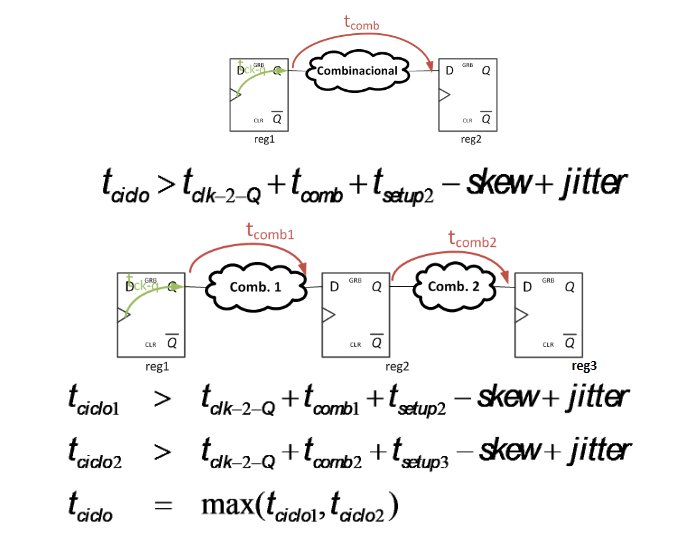
\includegraphics[width=0.7\textwidth]{images/Tema_2/segmentacion2.PNG}
	\caption{Tiempo de ciclo}
\end{figure}

\subsection{Rendimiento}
\textbf{Latencia:} tiempo transcurrido para obtener un nuevo resultado a la salida del circuito desde su entrada en este.
\[
	L = n*t_{ciclo}
\]
\textbf{Intervalo de inicialización (Throughput):} tasa de entrada de nuevos datos en el sistema por unidad de tiempo.
\[
	T = \frac{1}{t_{ciclo}}
\]

\section{Comportamiento dinámico}
La simulación lógica no mide retardos. Los retardos se miden en la Simulación Post-Place \& Route. La herramienta calcula el retardo de todos los caminos, el más lento, llamado camino crítico, es el que define el retardo del circuito. El retardo de los distintos caminos del circuito puede originar errores funcionales.

\subsection{Azares y glitches}
El retardo de propagación de un circuito se define como el tiempo necesario para obtener un valor de salida válido. Los azares o riesgos son las posibles fluctuaciones de la señal de salida antes de alcanzar su valor final:
\begin{itemize}
	\item Riesgo estático
	\item Riesgo dinámico
\end{itemize}
Estas fluctuaciones pueden ser uno o varios pulsos no deseados que reciben el nombre de glitches.

\subsection{Riesgos estáticos}
Un determinado cambio en la entrada produce un glitch en la salida cuando no debería producirse ningún cambio. Se deben a la existencia de distintos caminos que convergen hacia la salida con diferente retardo.

\subsection{Riesgos dinámicos}
La salida debe cambiar pero el cambio no es directo sino con fluctuaciones. Suelen producirse en circuitos con riesgo estático y un nivel más de puertas.

\subsection{Análisis de consumo}
Existen distintas métricas: potencia (temperatura) y  energía (duración de la batería).
Existe también el consumo estático y dinámico.

\subsection{Consumo estático}
Consumo de los bloques de circuito cuando no hay transiciones en las señales de entrada.
\[
	P_{static} = V_{dd} * I_{static}
\]
Donde:
\begin{itemize}
	\item $I_{static}$ es la corriente estática
	\item $V_{dd}$ es la tensión de alimentación
\end{itemize}

$I_{static}$ depende de la corriente de fuga de los transistores, la tensión de alimentación y la temperatura.

\subsection{Consumo dinámico}
Consumo de los bloques del circuito cuando hay transiciones en las señales de entrada.
\[
	P = \frac{1}{2}*C_{load}*V_{dd}^{2} * f * t
\]
Donde:
\begin{itemize}
	\item $C_{load}$ es la capacidad de carga
	\item $V_{dd}$ es la tensión de alimentación
	\item $f$ es la frecuencia del reloj
	\item $t$ es la tasa de actividad de la puerta
\end{itemize}
%finished
\chapterA{Diseño combinacional avanzado}
\section{Módulos combinacionales}

\subsection{Decodificador}
Circuito combinacional con n entradas y $2^{n}$ salidas. Cada salida es uno de los minterms que pueden generarse con n variables.
\[
	D_{i} =\left\{ \begin{array}{l}
		1\; si\; A=i donde\; A= \sum^{n-1}_{j=0}A_{j}2^{j}\; para\; 0 \leq i \leq 2^{n} -1 \\
		0 \; en \; caso \; contrario
	\end{array}\right\}
\]

\begin{figure}[H]
	\centering
	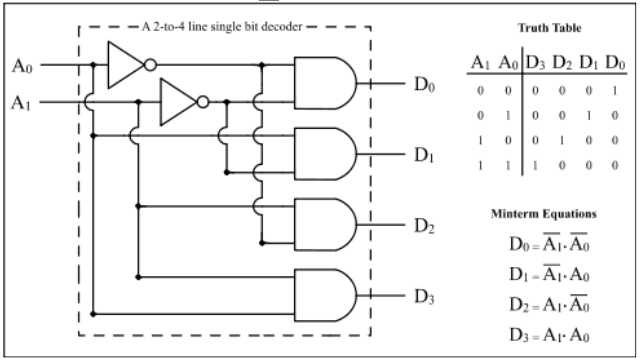
\includegraphics[width=0.8\textwidth]{images/Tema_3/Decodificador.PNG}
	\caption{Decodificador}
\end{figure}
\begin{figure}[H]
	\centering
	\lstinputlisting[style=customVHDL,  xleftmargin=.2\textwidth, xrightmargin=.2\textwidth]{Code/Tema_3/Decodificador.vhd}
	\caption{Código Codificador}
\end{figure}

\subsection{Decodificador}
\begin{figure}[H]
	\centering
	\lstinputlisting[style=customVHDL,  xleftmargin=.2\textwidth, xrightmargin=.2\textwidth]{Code/Tema_3/Codificador.vhd}
	\caption{Código Decodificador}
\end{figure}

\subsection{Multiplexor}

Descripción de alto nivel:
\[
	y = x_{s} \; donde \; s=\sum^{n-1}_{j=0} x_{j}2^{j}
\]

Implementación
\begin{itemize}
	\item 2 a 1 $y = x_{0} * \overline{s} + x_{1} * s$
	\item 4 a 1 $y = x_{0}\,\overline{s_{1}}\,\overline{s_{0}} + x_{1}\,\overline{s_{1}} \,s_{0} + x_{2}\,s_{1}\,\overline{s_{0}} + x_{3}\,s_{1}\,s_{0}$
\end{itemize}

\begin{figure}[H]
	\centering
	\lstinputlisting[style=customVHDL,  xleftmargin=.2\textwidth, xrightmargin=.2\textwidth]{Code/Tema_3/Multiplexor.vhd}
	\caption{Multiplexor}
\end{figure}
\newpage
\subsection{Sumador}
\begin{multicols}{2}
	\begin{figure}[H]
		\centering
		\lstinputlisting[style=customvhdl]{Code/Tema_3/Sumador1.vhd}
		\caption{Sumador con std\_logic}
	\end{figure}
	\vfill
	\null
	\begin{figure}[H]
		\centering
		\lstinputlisting[style=customvhdl]{Code/Tema_3/Sumador2.vhd}
		\caption{Sumador con numeric y datos con signo}
	\end{figure}
\end{multicols}

\begin{figure}[H]
	\centering
	\lstinputlisting[style=customvhdl]{Code/Tema_3/Restador.vhd}
	\caption{Restador}
\end{figure}


\section{Aritmética en VHDL}
\subsection{Operadores incluidos en VHDL-93 sin incluir ningún paquete}

\begin{table}[H]
	\begin{tabular}{|c|c|c|c|c|}
		\hline
		\rowcolor{gray}
		Operador & Descripción       & Tipo de operando a                          & Tipo de operando B                 & Tipo del resultado                 \\
		\hline
		a ** b   & Exponenciación    & Integer / Natural                           & Integer/ Natural                   & Integer / Natural                  \\
		\hline
		a * b    & Multiplicación    & \multirow{4}{*}{Integer / Natural}          & \multirow{4}{*}{Integer / Natural} & \multirow{4}{*}{Integer / Natural} \\
		\cline{1-2}
		a / b    & División          &                                             &                                    &                                    \\
		\cline{1-2}
		a mod b  & Módulo            &                                             &                                    &                                    \\
		\cline{1-2}
		a rem b  & Resto             &                                             &                                    &                                    \\
		\hline
		+ a      & Identidad         & \multirow{2}{*}{Integer / Natural}          &                                    & \multirow{2}{*}{Integer / Natural} \\
		\cline{1-2}
		- a      & Negación          &                                             &                                    &                                    \\
		\hline
		a + b    & Sumador           & \multirow{2}{*}{Integer / Natural}          & \multirow{2}{*}{Integer / Natural} & \multirow{2}{*}{Integer / Natural} \\
		\cline{1-2}
		a - b    & Resta             &                                             &                                    &                                    \\
		\hline
		a + b    & Concatenación     & Array 1-D, elemento                         & Array 1-D, elemento                & Array 1-D                          \\
		\hline
		a = b    & Igual             & \multirow{2}{*}{Cualquiera}                 & \multirow{2}{*}{Mismo que a}       & \multirow{2}{*}{boolean}           \\
		\cline{1-2}
		a /= b   & No igual          &                                             &                                    &                                    \\
		\hline
		a sll b  & Desp. Lóg. Izq.   & \multirow{6}{*}{bit\_vector}                & \multirow{6}{*}{Integer / Natural} & \multirow{6}{*}{bit\_vector}       \\
		\cline{1-2}
		a srl b  & Desp. Lóg. Der.   &                                             &                                    &                                    \\
		\cline{1-2}
		a sla b  & Desp. Arit. Der.  &                                             &                                    &                                    \\
		\cline{1-2}
		a sra b  & Desp. Arit. Der.  &                                             &                                    &                                    \\
		\cline{1-2}
		a rol b  & Rotación Izq.     &                                             &                                    &                                    \\
		\cline{1-2}
		a ror b  & Rotación der.     &                                             &                                    &                                    \\
		\hline
		a < b    & Menor que         & \multirow{4}{*}{Escalar o Array de 1-D}     & \multirow{4}{*}{Mismo que a}       & \multirow{4}{*}{boolean}           \\
		\cline{1-2}
		a <= b   & Menor o igual     &                                             &                                    &                                    \\
		\cline{1-2}
		a > b    & Mayor que         &                                             &                                    &                                    \\
		\cline{1-2}
		a >= b   & Mayor o igual que &                                             &                                    &                                    \\
		\hline
		a and b  & and               & \multirow{6}{*}{boolean, bit o bit\_vector} & \multirow{6}{*}{Mismo que a}       & \multirow{6}{*}{Mismo que a}       \\
		\cline{1-2}
		a or b   & or                &                                             &                                    &                                    \\
		\cline{1-2}
		a xor b  & xor               &                                             &                                    &                                    \\
		\cline{1-2}
		a nand b & nand              &                                             &                                    &                                    \\
		\cline{1-2}
		a nor b  & nor               &                                             &                                    &                                    \\
		\cline{1-2}
		a xnor b & xnor              &                                             &                                    &                                    \\
		\hline
	\end{tabular}
\end{table}

\subsection{Operadores y funciones del paquete IEEE std\_logic\_1164}
\begin{table}[H]
	\begin{tabular}{|c|c|c|c|}
		\hline
		\rowcolor{gray}
		Operador & Tipo de operando a                              & Tipo de operando b           & Tipo del resultado           \\
		\hline
		not a    & std\_logic\_vector, std\_logic                  &                              & Mismo que a                  \\
		\hline
		a and b  & \multirow{6}{*}{std\_logic\_vector, std\_logic} & \multirow{6}{*}{Mismo que a} & \multirow{6}{*}{Mismo que a} \\
		\cline{1-1}
		a or b   &                                                 &                              &                              \\
		\cline{1-1}
		a xor b  &                                                 &                              &                              \\
		\cline{1-1}
		a nand b &                                                 &                              &                              \\
		\cline{1-1}
		a nor b  &                                                 &                              &                              \\
		\cline{1-1}
		a xnor b &                                                 &                              &                              \\
		\hline
	\end{tabular}
\end{table}

\begin{table}[H]
	\begin{tabular}{|c|c|c|}
		\hline
		\rowcolor{gray}
		Función               & Tipo de operando a & Tipo de resultado \\
		\hline
		to\_bit(a)            & std\_logic         & bit               \\
		\hline
		to\_stdulogic(a)      & bit                & std\_logic        \\
		\hline
		to\_bitvector(a)      & std\_logic\_vector & bit\_vector       \\
		\hline
		to\_stdlogicvector(a) & bit\_vector        & std\_logi\_vector \\
		\hline
	\end{tabular}
\end{table}

\subsection{Operadores del paquete IEEE numeric\_std}
\begin{table}[H]
	\begin{tabular}{|c|c|c|c|}
		\hline
		\rowcolor{gray}
		Operador           & Tipo de operando a                                  & Tipo de operando b                                  & Tipo de resultado                 \\
		\hline
		abs a \newline - a & signed                                              &                                                     & signed                            \\
		\hline
		a * b              & \multirow{6}{*}{unsigned, natural, signed, integer} & \multirow{6}{*}{unsigned, natural, signed, integer} & \multirow{6}{*}{unsigned, signed} \\
		\cline{1-1}
		a / b              &                                                     &                                                     &                                   \\
		\cline{1-1}
		a mod b            &                                                     &                                                     &                                   \\
		\cline{1-1}
		a rem b            &                                                     &                                                     &                                   \\
		\cline{1-1}
		a + b              &                                                     &                                                     &                                   \\
		\cline{1-1}
		a - b              &                                                     &                                                     &                                   \\
		\hline
		a = b              & \multirow{6}{*}{unsigned, natural, signed, integer} & \multirow{6}{*}{unsigned, natural, signed, integer} & \multirow{6}{*}{boolean}          \\
		\cline{1-1}
		a /= b             &                                                     &                                                     &                                   \\
		\cline{1-1}
		a < b              &                                                     &                                                     &                                   \\
		\cline{1-1}
		a <= b             &                                                     &                                                     &                                   \\
		\cline{1-1}
		a > b              &                                                     &                                                     &                                   \\
		\cline{1-1}
		a >= b             &                                                     &                                                     &                                   \\
		\hline
	\end{tabular}
\end{table}

\subsection{Funciones de conversión de datos o casting}
Para la conversión de señales de un tipo a otro se deben usar las siguientes funciones y operaciones de casting:

\begin{figure}[H]
	\centering
	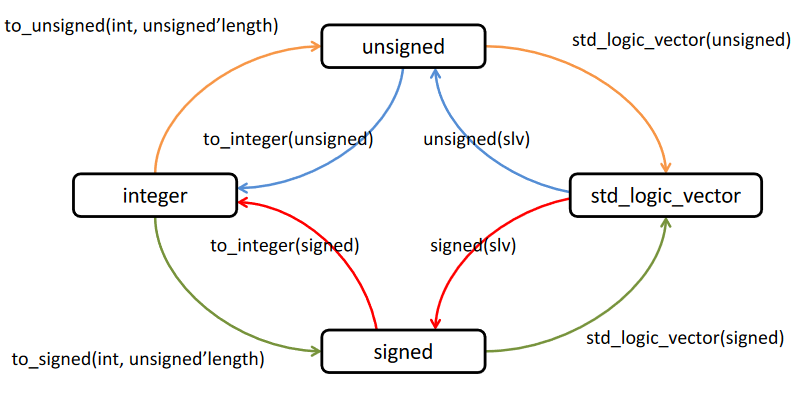
\includegraphics[width=0.9\textwidth]{images/Tema_3/casting.PNG}
	\caption{Funciones de conversión de tipos}
\end{figure}
\section{Unidades funcionales multifunción}
En este apartado se estudia la estructura del diseño y reducir la cantidad de recursos \gls{hw} compartiendo lógica entre distintas operaciones.\\
Para ello agruparemos \gls{uf} sencillas en \gls{uf} más complejas, esto se conoce como \gls{uf} multifunción. Esto lo utilizaremos cuando la \gls{uf} multifunción y el coste de conexión es menor que el coste de las \gls{uf} sencillas. Para lograr esto utilizaremos un algoritmo de particionamiento y un grafo de compatibilidad.
\begin{figure}[H]
	\centering
	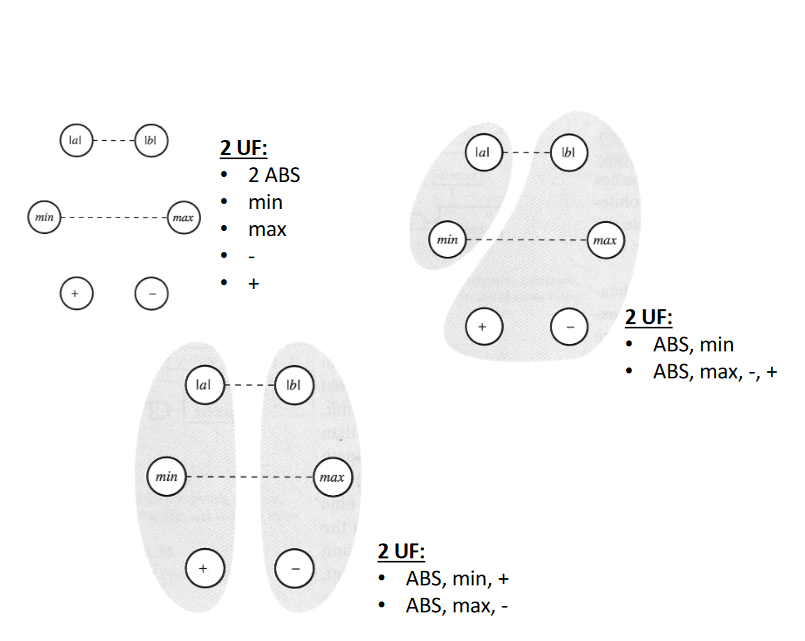
\includegraphics[width=0.5\textwidth]{images/Tema_3/Optimizacion.PNG}
	\caption{Optimización de múltiples \gls{uf}}
\end{figure}

\section{Redes iterativas}
Las redes iterativas son conjuntos de módulos idénticos, cada uno conectado exclusivamente a los módulos vecinos.

Una red iterativa 1-D de orden k es una implementación de una función de n variables, donde:
\begin{itemize}
	\item (n/k) celdas idénticas, G, con:
	      \begin{itemize}
		      \item Entradas externas x, e internas c
		      \item Salidas externas z, e internas c
	      \end{itemize}
	      \[
		      C_{j+1}=G\left(x_{j},c_{j}\right)
	      \]
	      \[
		      Z_{j}=F\left(x_{j}, c_{j}\right)
	      \]

	\item Celdas de los extremos pueden simplificarse aprovechando las condiciones de contorno
	      \begin{figure}[H]
		      \centering
		      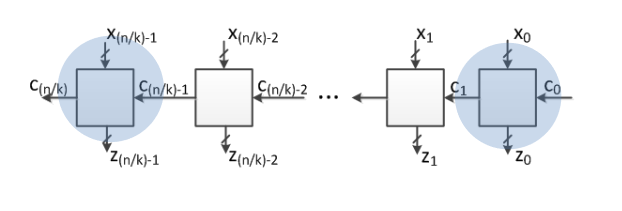
\includegraphics[width=0.6\textwidth]{images/Tema_3/Ejemplo_RI.PNG}
		      \caption{Ejemplo Red Iterativa 1-D}
	      \end{figure}
\end{itemize}

\subsection{Diseño}
Primero determinamos el valor de k, el equilibrio entre la complejidad de las celdas (nº de entradas) y el nº de celdas (retardo total).\\
Después determinamos los valores que deben trasmitirse entre los módulos intermedios (salidas internas) y el valor de la salida externa del último módulo. \\
Finalmente hacemos la descripción de alto nivel de los bloques intermedios, la implementación de las funciones de conmutación de los bloques, y la simplificación de las celdas inicial y final.

\subsection{Temporización}
Retardo $\left(\Delta\right)$
\begin{itemize}
	\item Función de retardo de las salidas externas de cada celda $\Delta_{o}$
	\item Función de retardo de las salidas internas de cada celda $\Delta_{c}$
\end{itemize}
\[
	\Delta = \left(\frac{n}{k}-1\right)\Delta_{c}+max\left(\Delta_{o}, \Delta_{c}\right)
\]

\subsection{Redes 1-D en VHDL}
En este ejemplo se diseñará una red de resolución de propiedades iterativa con n entradas y n salidas. LA salida $Z_{i} = 1\; si\; X_{i}= 1\; y\; X_{j} \forall j>i$

\begin{multicols}{2}
	\begin{figure}[H]
		\centering
		\lstinputlisting[style=customVHDL]{Code/Tema_3/Ejemplo_Celda_1.vhd}
		\caption{Ejemplo de celda de la red}
	\end{figure}
	\vfill
	\null
	\begin{figure}[H]
		\centering
		\lstinputlisting[style=customVHDL]{Code/Tema_3/Ejemplo_Array_Celdas_1.vhd}
		\caption{Generador de celdas conectadas}
	\end{figure}
\end{multicols}
\begin{figure}[H]
	\centering
	\lstinputlisting[style=customVHDL]{Code/Tema_3/Ejemplo_Red_1.vhd}
	\caption{Ejemplo red iterativa con generate}
\end{figure}

\subsection{Redes iterativas 2-D}
Array de celdas idénticas conectadas con sus vecinas. Cada celda (i,j) posee:
\begin{figure}[H]
	\centering
	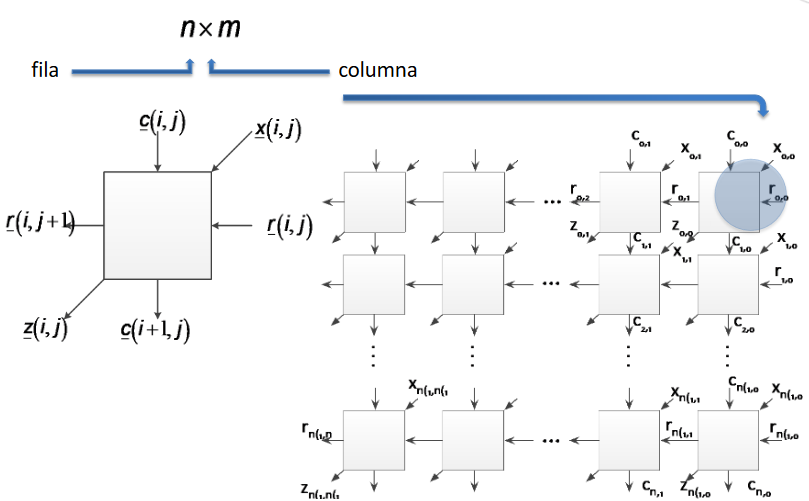
\includegraphics[width=\textwidth]{images/Tema_3/Red_2D.PNG}
\end{figure}

Para generar una matriz 2D tendremos que usar dos bucles anidados.

\section{Técnicas de mejora del rendimiento}
La utilización de diseños combinacionales bastante grandes (datos de entrada a partir de 32 bits), hace que el tiempo asociado al cambio crítico sea grande y el retardo de la red elevado.\\
En las redes iterativas la última celda no podrá generar su salida hasta que no haya recibido su señal intermedia. Esta señal interna ha tenido que atravesar n - 1 celdas que componen la red, por lo tanto el retardo es muy elevado si n es grande.

\subsection{Redes de anticipación}
Para reducir el retardo de las redes iterativas, anticiparemos el valor de la señal que se propaga entre celdas.

\begin{figure}[H]
	\centering
	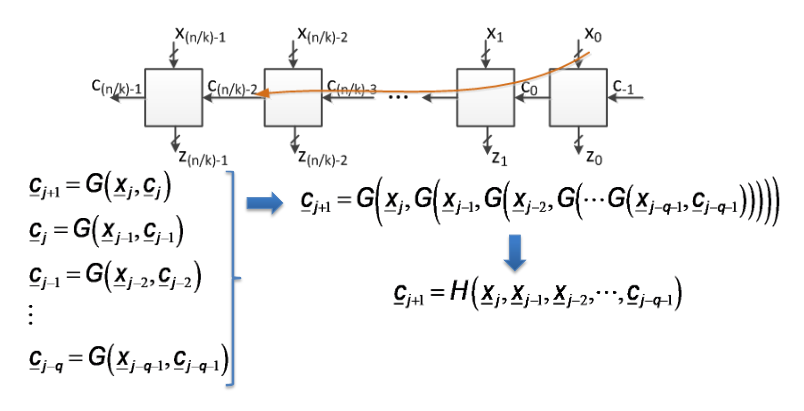
\includegraphics[width=\textwidth]{images/Tema_3/Redes_Anticipacion_1.PNG}
	\caption{Red iterativa sin anticipación}
\end{figure}
\begin{figure}[H]
	\centering
	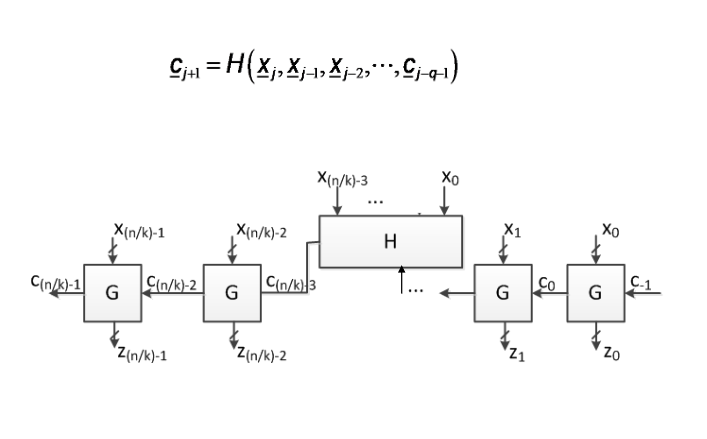
\includegraphics[width=\textwidth]{images/Tema_3/Redes_Anticipacion_2.PNG}
	\caption{Red iterativa con anticipación}
\end{figure}
\newpage
\subsection{Redes en árbol}
Implementar una función de n entradas usando bloques de k entradas:
\begin{figure}[H]
	\centering
	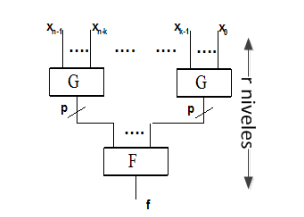
\includegraphics[width=0.5\textwidth]{images/Tema_3/Red_Arbol.PNG}
	\caption{Red en árbol}
\end{figure}
\begin{itemize}
	\item Módulo G: k entradas y p salidas $\rightarrow \frac{n}{k}$ módulos
	\item Módulo F: $p\frac{n}{k}$ entradas
	\item Retardo: $\left(r - 1\right)\Delta_{G} + \Delta_{F}$
\end{itemize}

\section{Errores de diseño}
\subsection{Lazos combinacionales}
Estructuras lógicas que contienen realimentación sin ningún elemento síncrono en el camino. Por ejemplo \textcolor{blue}{$A <= A + 1;$} \gls{vhdl} no permitirá ni la simulación ni la síntesis de este diseño.
\subsection{Errores de diseño en circuitos combinacionales}
Si implementamos la lógica combinacional mediante un process:
\begin{itemize}
	\item\textbf{Error 1:} no incluir todas las entradas en la lista de sensibilidad
	\item\textbf{Error 2:} no terminar una sentencia if con un else
	\item\textbf{Error 3:} no especificar el valor de alguna salida en alguna de las ramas de la sentencia if
\end{itemize}

En los errores 2 y 3 se añadirá un latch, lo que implica lógica secuencial.
%finished
\chapterA{Diseño algorítmico}
\section{Introducción}
\begin{figure}[H]
	\centering
	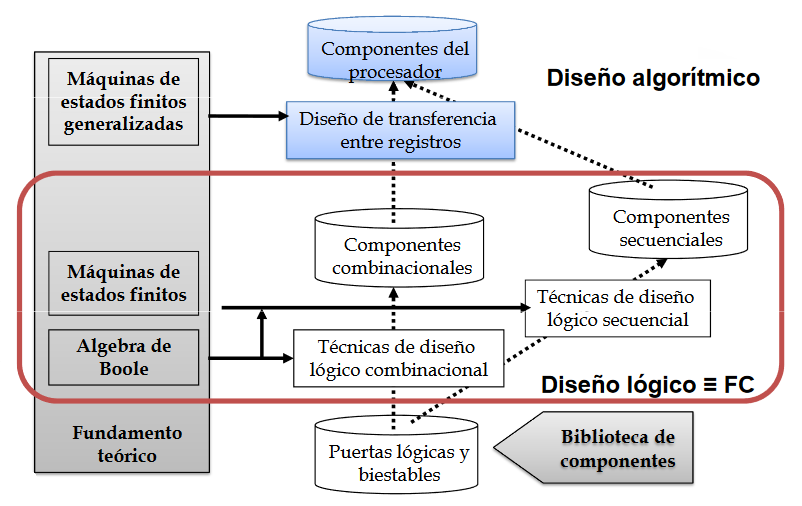
\includegraphics[width=\textwidth]{images/Tema_4/Flujo_Diseno.PNG}
	\caption{Flujo de diseño}
\end{figure}


\printglossary[title=Glosario]

\let\cleardoublepage\clearpage
\listoffigures
\addcontentsline{toc}{chapter}{Índice de figuras}
\let\cleardoublepage\clearpage

\listoftables
\addcontentsline{toc}{chapter}{Índice de cuadros}
\end{document}
